%
% mathpendel.tex -- Das mathematische Pendel
%
% (c) 2022 Prof Dr Andreas Müller, OST Ostschweizer Fachhochschule
%

\subsection{Das mathematische Pendel
\label{buch:elliptisch:subsection:mathpendel}}
\begin{figure}
\centering
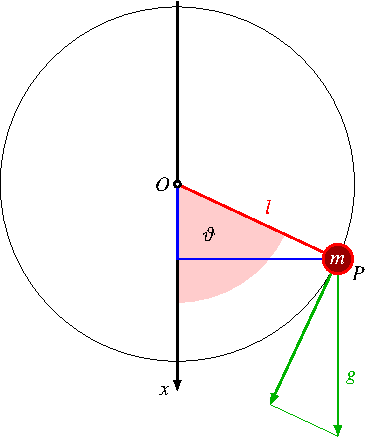
\includegraphics{chapters/110-elliptisch/images/pendel.pdf}
\caption{Mathematisches Pendel
\label{buch:elliptisch:fig:mathpendel}}
\end{figure}
Das in Abbildung~\ref{buch:elliptisch:fig:mathpendel} dargestellte
Mathematische Pendel besteht aus einem Massepunkt der Masse $m$
im Punkt $P$,
der über eine masselose Stange der Länge $l$ mit dem Drehpunkt $O$
verbunden ist.
Das Pendel bewegt sich unter dem Einfluss der Schwerebeschleunigung $g$.

Das Trägheitsmoment des Massepunktes um den Drehpunkt $O$ ist
\(
I=ml^2
\).
Das Drehmoment der Schwerkraft ist
\(M=gl\sin\vartheta\).
Die Bewegungsgleichung wird daher
\[
\begin{aligned}
\frac{d}{dt} I\dot{\vartheta}
&=
M
=
gl\sin\vartheta
\\
ml^2\ddot{\vartheta}
&=
gl\sin\vartheta
&&\Rightarrow&
\ddot{\vartheta}
&=\frac{g}{l}\sin\vartheta
\end{aligned}
\]
Dies ist eine nichtlineare Differentialgleichung zweiter Ordnung, die
wir nicht unmittelbar mit den Differentialgleichungen erster Ordnung
der elliptischen Funktionen vergleichen können.

Die Differentialgleichungen erster Ordnung der elliptischen Funktionen
enthalten das Quadrat der ersten Ableitung.
In unserem Fall entspricht das einer Gleichung, die $\dot{\vartheta}^2$
enthält.
Der Energieerhaltungssatz kann uns eine solche Gleichung geben.
Die Summe von kinetischer und potentieller Energie muss konstant sein.
Dies führt auf
\[
E_{\text{kinetisch}}
+
E_{\text{potentiell}}
=
\frac12I\dot{\vartheta}^2
+
mgl(1-\cos\vartheta)
=
\frac12ml^2\dot{\vartheta}^2
+
mgl(1-\cos\vartheta)
=
E
\]
Durch Auflösen nach $\dot{\vartheta}$ kann man jetzt die
Differentialgleichung
\[
\dot{\vartheta}^2
=
-
\frac{2g}{l}(1-\cos\vartheta)
+\frac{2E}{ml^2}
\]
finden.
In erster Näherung, d.h. wenn man die rechte Seite bis zu vierten
Potenzen in eine Taylor-Reihe in $\vartheta$ entwickelt,  ist dies
tatsächlich eine Differentialgleichung der Art, wie wir sie für
elliptische Funktionen gefunden haben, wir möchten aber eine exakte
Lösung konstruieren.

Die maximale Energie für eine Bewegung, bei der sich das Pendel gerade
über den höchsten Punkt hinweg zu bewegen vermag, ist 
$E=2lmg$.
Falls $E<2mgl$ ist, erwarten wir Schwingungslösungen, bei denen 
der Winkel $\vartheta$ immer im offenen Interval $(-\pi,\pi)$
bleibt.
Für $E>2mgl$ wird sich das Pendel im Kreis bewegen, für sehr grosse
Energie ist die kinetische Energie dominant, die Verlangsamung im
höchsten Punkt wird immer weniger ausgeprägt sein.

%
% Koordinatentransformation auf elliptische Funktionen
%
\subsubsection{Koordinatentransformation auf elliptische Funktionen}
Wir verwenden als neue Variable 
\[
y = \sin\frac{\vartheta}2
\]
mit der Ableitung
\[
\dot{y}=\frac12\cos\frac{\vartheta}{2}\cdot \dot{\vartheta}.
\]
Man beachte, dass $y$ nicht eine Koordinate in
Abbildung~\ref{buch:elliptisch:fig:mathpendel} ist.

Aus den Halbwinkelformeln finden wir
\[
\cos\vartheta
=
1-2\sin^2 \frac{\vartheta}2
=
1-2y^2.
\]
Dies können wir zusammen mit der
Identität $\cos^2\vartheta/2 = 1-\sin^2\vartheta/2 = 1-y^2$
in die Energiegleichung einsetzen und erhalten
\[
\frac12ml^2\dot{\vartheta}^2 + mgly^2 = E
\qquad\Rightarrow\qquad
\frac14 \dot{\vartheta}^2 = \frac{E}{2ml^2} - \frac{g}{2l}y^2.
\]
Der konstante Term auf der rechten Seite ist grösser oder kleiner als
$1$ je nachdem, ob das Pendel sich im Kreis bewegt oder nicht.

Durch Multiplizieren mit $\cos^2\frac{\vartheta}{2}=1-y^2$
erhalten wir auf der linken Seite einen Ausdruck, den wir
als Funktion von $\dot{y}$ ausdrücken können.
Wir erhalten
\begin{align*}
\frac14
\cos^2\frac{\vartheta}2
\cdot
\dot{\vartheta}^2
&=
\frac14
(1-y^2)
\biggl(\frac{E}{2ml^2} -\frac{g}{2l}y^2\biggr)
\\
\dot{y}^2
&=
\frac{1}{4}
(1-y^2)
\biggl(\frac{E}{2ml^2} -\frac{g}{2l}y^2\biggr)
\end{align*}
Die letzte Gleichung hat die Form einer Differentialgleichung
für elliptische Funktionen.
Welche Funktion verwendet werden muss, hängt von der Grösse der
Koeffizienten in der zweiten Klammer ab.
Die Tabelle~\ref{buch:elliptisch:tabelle:loesungsfunktionen}
zeigt, dass in der zweiten Klammer jeweils einer der Terme
$1$ sein muss.

%
% Der Fall E < 2mgl
%
\subsubsection{Der Fall $E<2mgl$}
\begin{figure}
\centering
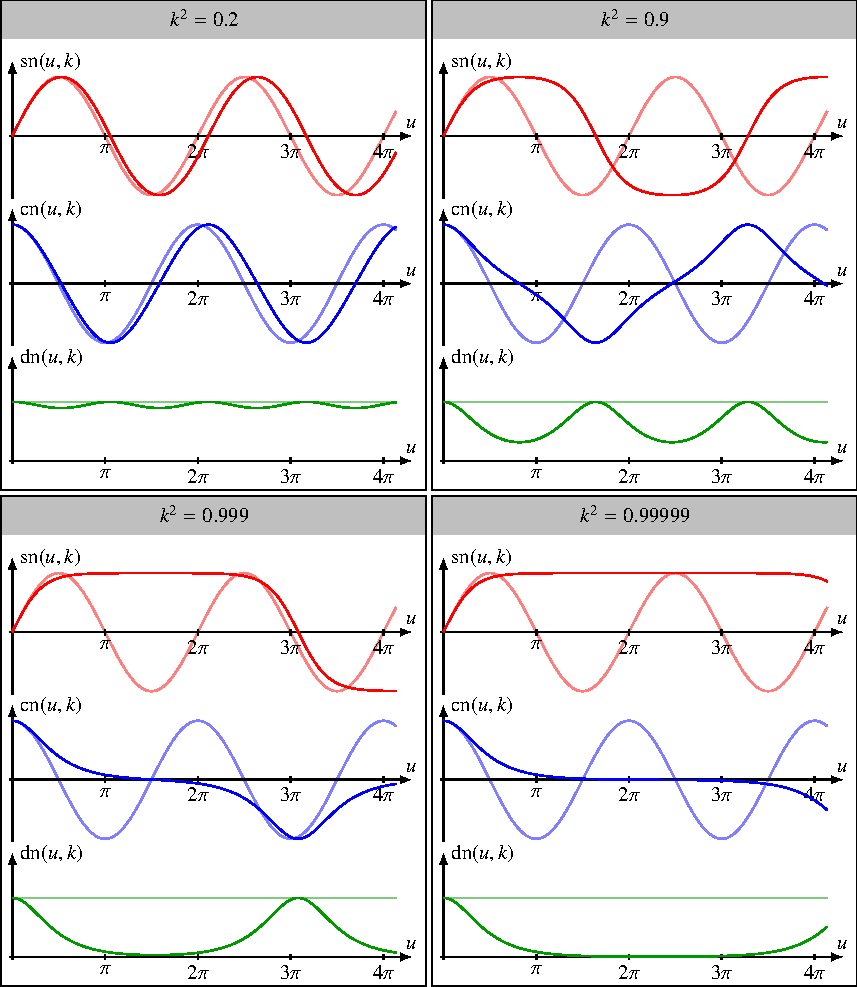
\includegraphics[width=\textwidth]{chapters/110-elliptisch/images/jacobiplots.pdf}
\caption{%
Abhängigkeit der elliptischen Funktionen von $u$ für
verschiedene Werte von $k^2=m$.
Für $m=0$ ist $\operatorname{sn}(u,0)=\sin u$, 
$\operatorname{cn}(u,0)=\cos u$ und $\operatorname{dn}(u,0)=1$, diese
sind in allen Plots in einer helleren Farbe eingezeichnet.
Für kleine Werte von $m$ weichen die elliptischen Funktionen nur wenig
von den trigonometrischen Funktionen ab,
es ist aber klar erkennbar, dass die anharmonischen Terme in der
Differentialgleichung die Periode mit steigender Amplitude verlängern.
Sehr grosse Werte von $m$ nahe bei $1$ entsprechen der Situation, dass
die Energie des Pendels fast ausreicht, dass es den höchsten Punkt
erreichen kann, was es für $m$ macht.
\label{buch:elliptisch:fig:jacobiplots}}
\end{figure}


Wir verwenden als neue Variable 
\[
y = \sin\frac{\vartheta}2
\]
mit der Ableitung
\[
\dot{y}=\frac12\cos\frac{\vartheta}{2}\cdot \dot{\vartheta}.
\]
Man beachte, dass $y$ nicht eine Koordinate in
Abbildung~\ref{buch:elliptisch:fig:mathpendel} ist.

Aus den Halbwinkelformeln finden wir
\[
\cos\vartheta
=
1-2\sin^2 \frac{\vartheta}2
=
1-2y^2.
\]
Dies können wir zusammen mit der
Identität $\cos^2\vartheta/2 = 1-\sin^2\vartheta/2 = 1-y^2$
in die Energiegleichung einsetzen und erhalten
\[
\frac12ml^2\dot{\vartheta}^2 + mgly^2 = E.
\]
Durch Multiplizieren mit $\cos^2\frac{\vartheta}{2}=1-y^2$
erhalten wir auf der linken Seite einen Ausdruck, den wir
als Funktion von $\dot{y}$ ausdrücken können.
Wir erhalten
\begin{align*}
\frac12ml^2
\cos^2\frac{\vartheta}2
\dot{\vartheta}^2
&=
(1-y^2)
(E -mgly^2)
\\
\frac{1}{4}\cos^2\frac{\vartheta}{2}\dot{\vartheta}^2
&=
\frac{1}{2}
(1-y^2)
\biggl(\frac{E}{ml^2} -\frac{g}{l}y^2\biggr)
\\
\dot{y}^2
&=
\frac{E}{2ml^2}
(1-y^2)\biggl(
1-\frac{2gml}{E}y^2
\biggr).
\end{align*}
Dies ist genau die Form der Differentialgleichung für die elliptische
Funktion $\operatorname{sn}(u,k)$
mit $k^2 = 2gml/E< 1$.

%%
%% Der Fall E > 2mgl
%%
%\subsection{Der Fall $E > 2mgl$}
%In diesem Fall hat das Pendel im höchsten Punkte immer noch genügend
%kinetische Energie, so dass es sich im Kreise dreht.
%Indem wir die Gleichung


%\subsection{Soliton-Lösungen der Sinus-Gordon-Gleichung}

%\subsection{Nichtlineare Differentialgleichung vierter Ordnung}
%XXX Möbius-Transformation \\
%XXX Reduktion auf die Differentialgleichung elliptischer Funktionen
